% Chapter Template

\chapter{Ensayos y Resultados} % Main chapter title

\label{Chapter4} % Change X to a consecutive number; for referencing this chapter elsewhere, use \ref{ChapterX}

En este capítulo se describe la estrategia general de \textit{testing} del proyecto y se documentan los ensayos realizados en 3 niveles de abstracción: a nivel de función, a nivel de módulo y a nivel de sistema.

%----------------------------------------------------------------------------------------
%	SECTION 1
%----------------------------------------------------------------------------------------

\section{Test Master Plan}
\label{sec:masterPlan}

Para la elaboración de un \textit{Test Master Plan} se tomaron elementos del paradigma de desarrollo basado el pruebas o TDD (por sus siglas en inglés, \textit{Test Driven Development}) como fue mencionado en la subsección \ref{subsec:tdd}. 

Cabe destacar que en la planificación de las tareas del proyecto, primero se definieron los casos de prueba; luego se prepararon las herramientas de \textit{testing}; luego se implementaron los módulos y finalmente, se realizaron las pruebas. Esto puede observarse en el diagrama de \textit{Activity on Node} de la figura \ref{fig:AoN} en la sección \ref{sec:plan}.

En ese sentido, resultó necesario tener bien definidos los requisitos funcionales y sus criterios de aceptación.  Se debieron contemplar todos los casos posibles de uso, tanto exitosos como de error, con lo que se elaboró un documento \citep{TestMasterPlan} de casos de prueba por módulo  y de esta manera, se dio cumplimiento al requerimiento 1.2 indicado en la sección \ref{sec:requerimientos}.  

Se ensayó el código en 3 niveles distintos de abstracción: a nivel de función, de módulo y de sistema, según se documenta en las subsecciones \ref{subsec:unitarias}, \ref{subsec:pruebasFuncionales} y \ref{subsec:pruebasSistema}, respectivamente. 

Asimismo, las pruebas sobre los módulos fueron diseñadas para evaluar únicamente la lógica principal de funcionamiento.  En cada caso, se debió abstraer al módulo bajo ensayo de otras capas o servicios que pudieran interactuar con su lógica principal, para lo cual se simuló el resultado de dichas interacciones con \textit{mocks}. 


\subsection{Pruebas unitarias}
\label{subsec:unitarias}

[\textbf{hablar de ceedling}]

\begin{figure}[ht]
	\centering
	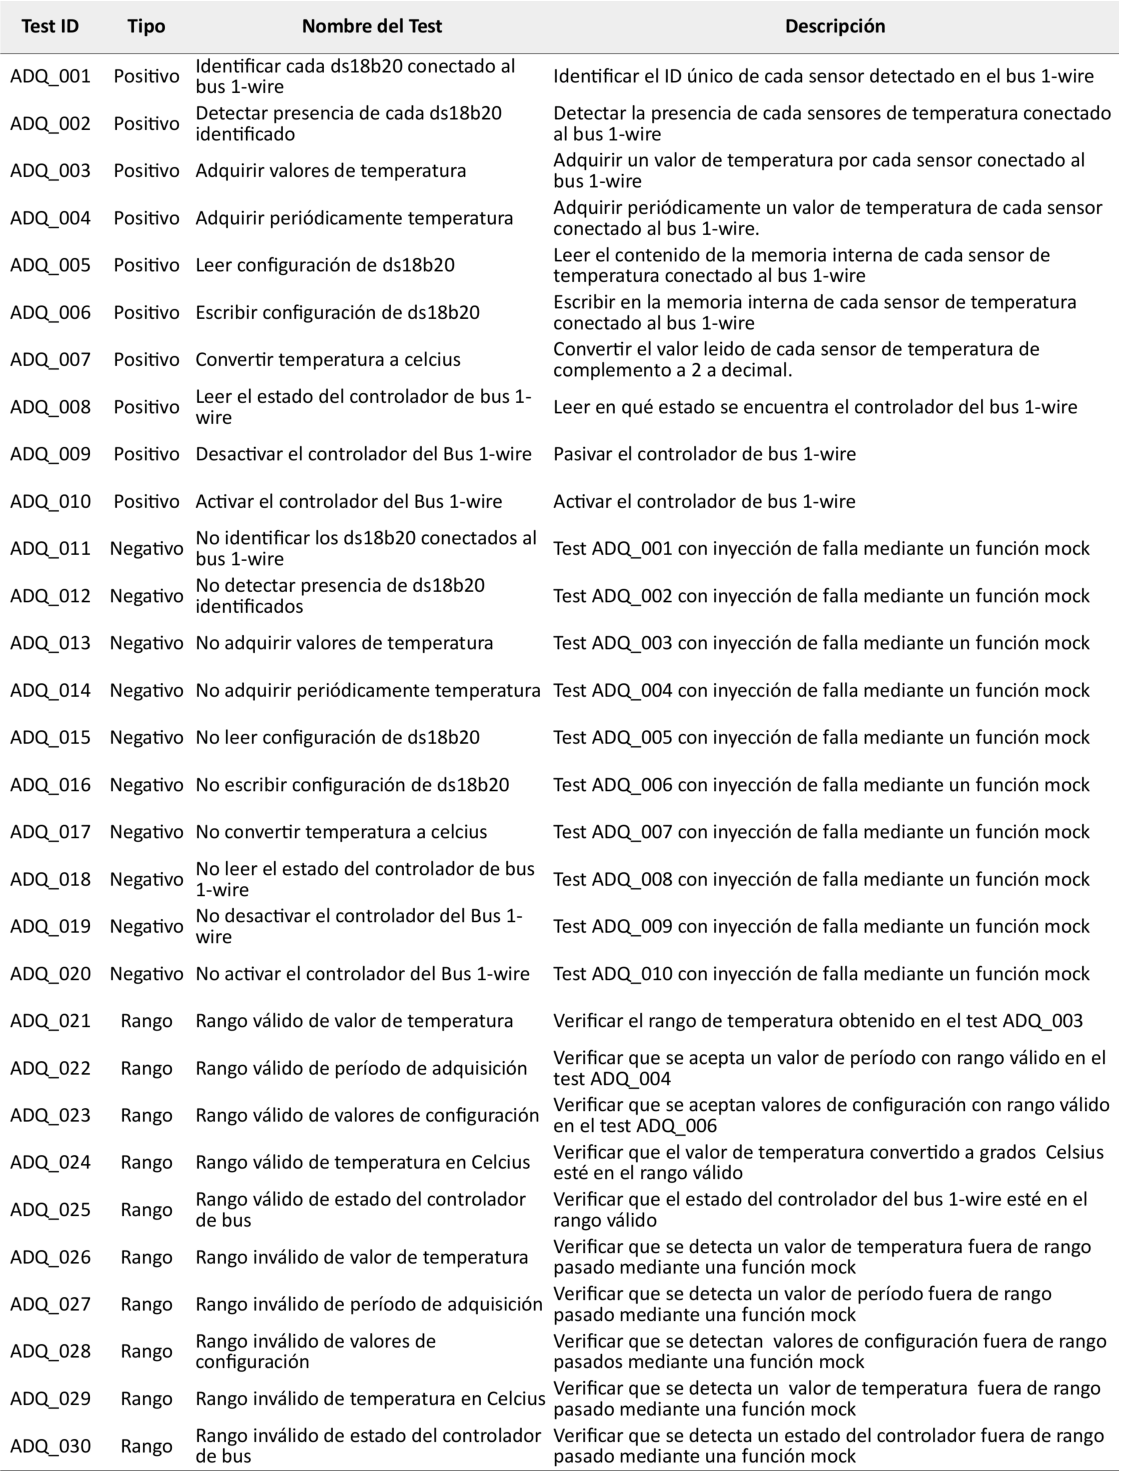
\includegraphics[width=\textwidth]{./Figures/TestADQ.pdf}
	\caption{algo}
	\label{fig:IPfC}
\end{figure}

\begin{figure}[ht]
	\centering
	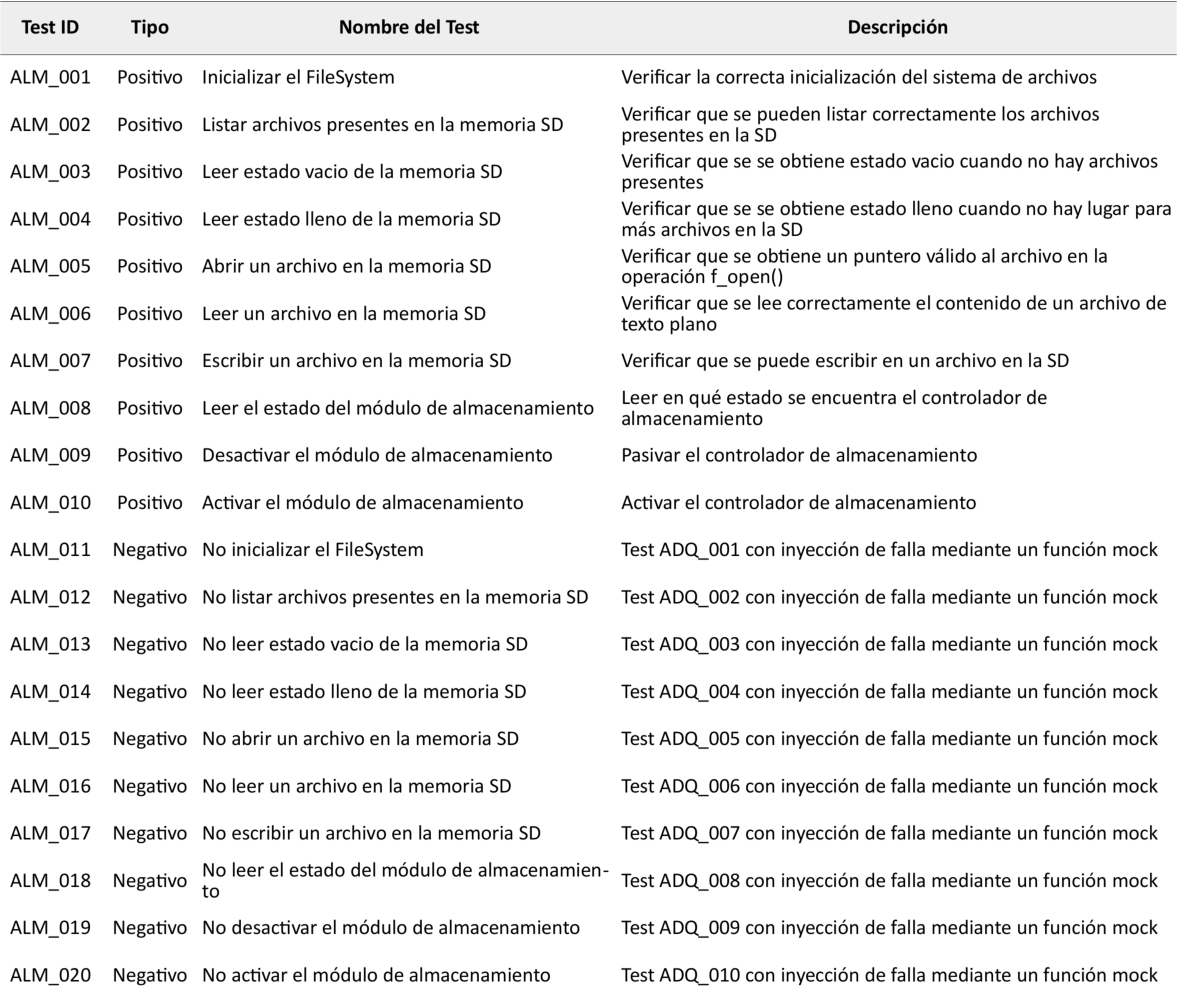
\includegraphics[width=\textwidth]{./Figures/TestSD.pdf}
	\caption{algo}
	\label{fig:IPfC}
\end{figure}

\subsection{Pruebas funcionales}
\label{subsec:pruebasFuncionales}


[\textbf{pruebas sobre las MEF de cada bloque}]

\subsection{Pruebas de sistema}
\label{subsec:pruebasSistema}

[\textbf{Pruebas}]